\documentclass{beamer}

\usepackage{graphicx}
\usepackage[utf8]{inputenc}

\title{GCM; The illegal attack}
\author{Mathias Hall-Andersen (rot256)}
\institute{Pwnies @ Copenhagen University}
\date{2017}

\begin{document}

\frame{\titlepage}

\begin{frame}
\frametitle{Authenticated encryption}
Why
\end{frame}

\begin{frame}
\frametitle{Galois Counter Mode (motivation)}
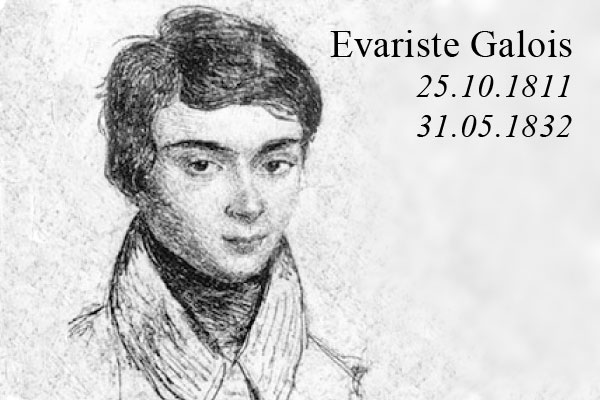
\includegraphics[width=\textwidth]{evariste_galois}
\end{frame}

\begin{frame}
\frametitle{Some algebra}
\end{frame}

\begin{frame}
\frametitle{Rings}
\[
    \mathbb{Z}
\]
\end{frame}

\begin{frame}
\frametitle{Fields}
\[
    \mathbb{Q}, \mathbb{R}
\]
\end{frame}

\begin{frame}
\frametitle{Rings \& Fields}
We will primarily be dealing with the field of two elements:
$1, 0$ \\
Where:
\begin{align}
    1 \cdot x &= x \text{ : 1 is the multiplicative identity} \\
    0 + x     &= x \text{ : 0 is the additive identity} \\
    1 + 1     &= 0 \text{ : the field has characteristic 2}
\end{align}
No magic.
Question:
If considered like bits, what common operations does
addition and multiplication in the field correspond to?
What implication does it have for bit-slicing techniques?
\end{frame}

\begin{frame}
\frametitle{Polynomials over Rings}
\end{frame}

\begin{frame}
\frametitle{Galois Counter Mode (operation)}
\end{frame}

\begin{frame}
\frametitle{SageMath}
`SageMath is a free open-source mathematics software system licensed under the GPL.
 It builds on top of many existing open-source packages:
 NumPy, SciPy, matplotlib, Sympy, Maxima, GAP, FLINT, R and many more'
 - \url{https://www.sagemath.org/}
\end{frame}

\begin{frame}
\frametitle{SageMath}
sage or go to \url{https://cocalc.com/app}
\end{frame}


\begin{frame}
\frametitle{Nonce reuse attack}
Theorists \& mathematicians care about proofs. \\
Hackers care about assumptions.
\end{frame}

\begin{frame}
\frametitle{Work session}
\end{frame}

\begin{frame}
\frametitle{Truncated nonce attack}
\end{frame}

\end{document}
